\chapter{Introdução}
\label{c_introducao}

A depuração é entendida como um dos conceitos centrais do aprendizado de programação \cite{carver_assessing_1986}. Ela compreende a etapa de encontrar e solucionar problemas (\textit{bugs}\footnote{
    Termo em inglês que, quando ligado à informática, significa falha ou defeito em código que provoca mau funcionamento.
}) em um algoritmo. \citeonline{mccauley_debugging_2008} menciona que há grande quantidade de literatura sobre o tema, que é considerado de difícil aprendizado pelos estudantes e um desafio de ensino para os professores. Essa literatura busca responder questões como: Quais as causas dos \textit{bugs}?, Que tipos de \textit{bugs} ocorrem? e Como melhorar o ensino e aprendizado de depuração?

Enquanto no contexto comercial os \textit{bugs} de \textit{software} são indesejados e causam enormes prejuízos de toda ordem \cite{valdivia-garcia_understanding_2016}, no contexto educacional eles representam uma oportunidade de aprendizado. Segundo \citeonline{papert_mindstorms:_1980}, não se espera que qualquer coisa funcione na primeira tentativa, e portanto errar e depurar faz parte do processo. 

\citeonline{valente_aspectos_2018} expressa essa ideia como uma espiral de \textit{descrição-execução-reflexão-depuração} (\autoref{fig_espiral}). Ao entrar nessa espiral, primeiramente o aluno descreve um programa e o executa, a fim de obter um resultado. Pode, então, refletir sobre se a execução do seu programa resultou naquilo que intencionava. Por fim, em caso negativo, deve depurar o programa. Essa depuração pode eliminar erros de sintaxe, revelar incompreensão de conceitos envolvidos no problema ou esclarecer quais passos devem ser aplicados para resolvê-lo. Esse ciclo possibilita ao aluno passar de um nível de conhecimento inicial para outro mais elaborado.

\begin{figure}[!htpb]
  \centering
  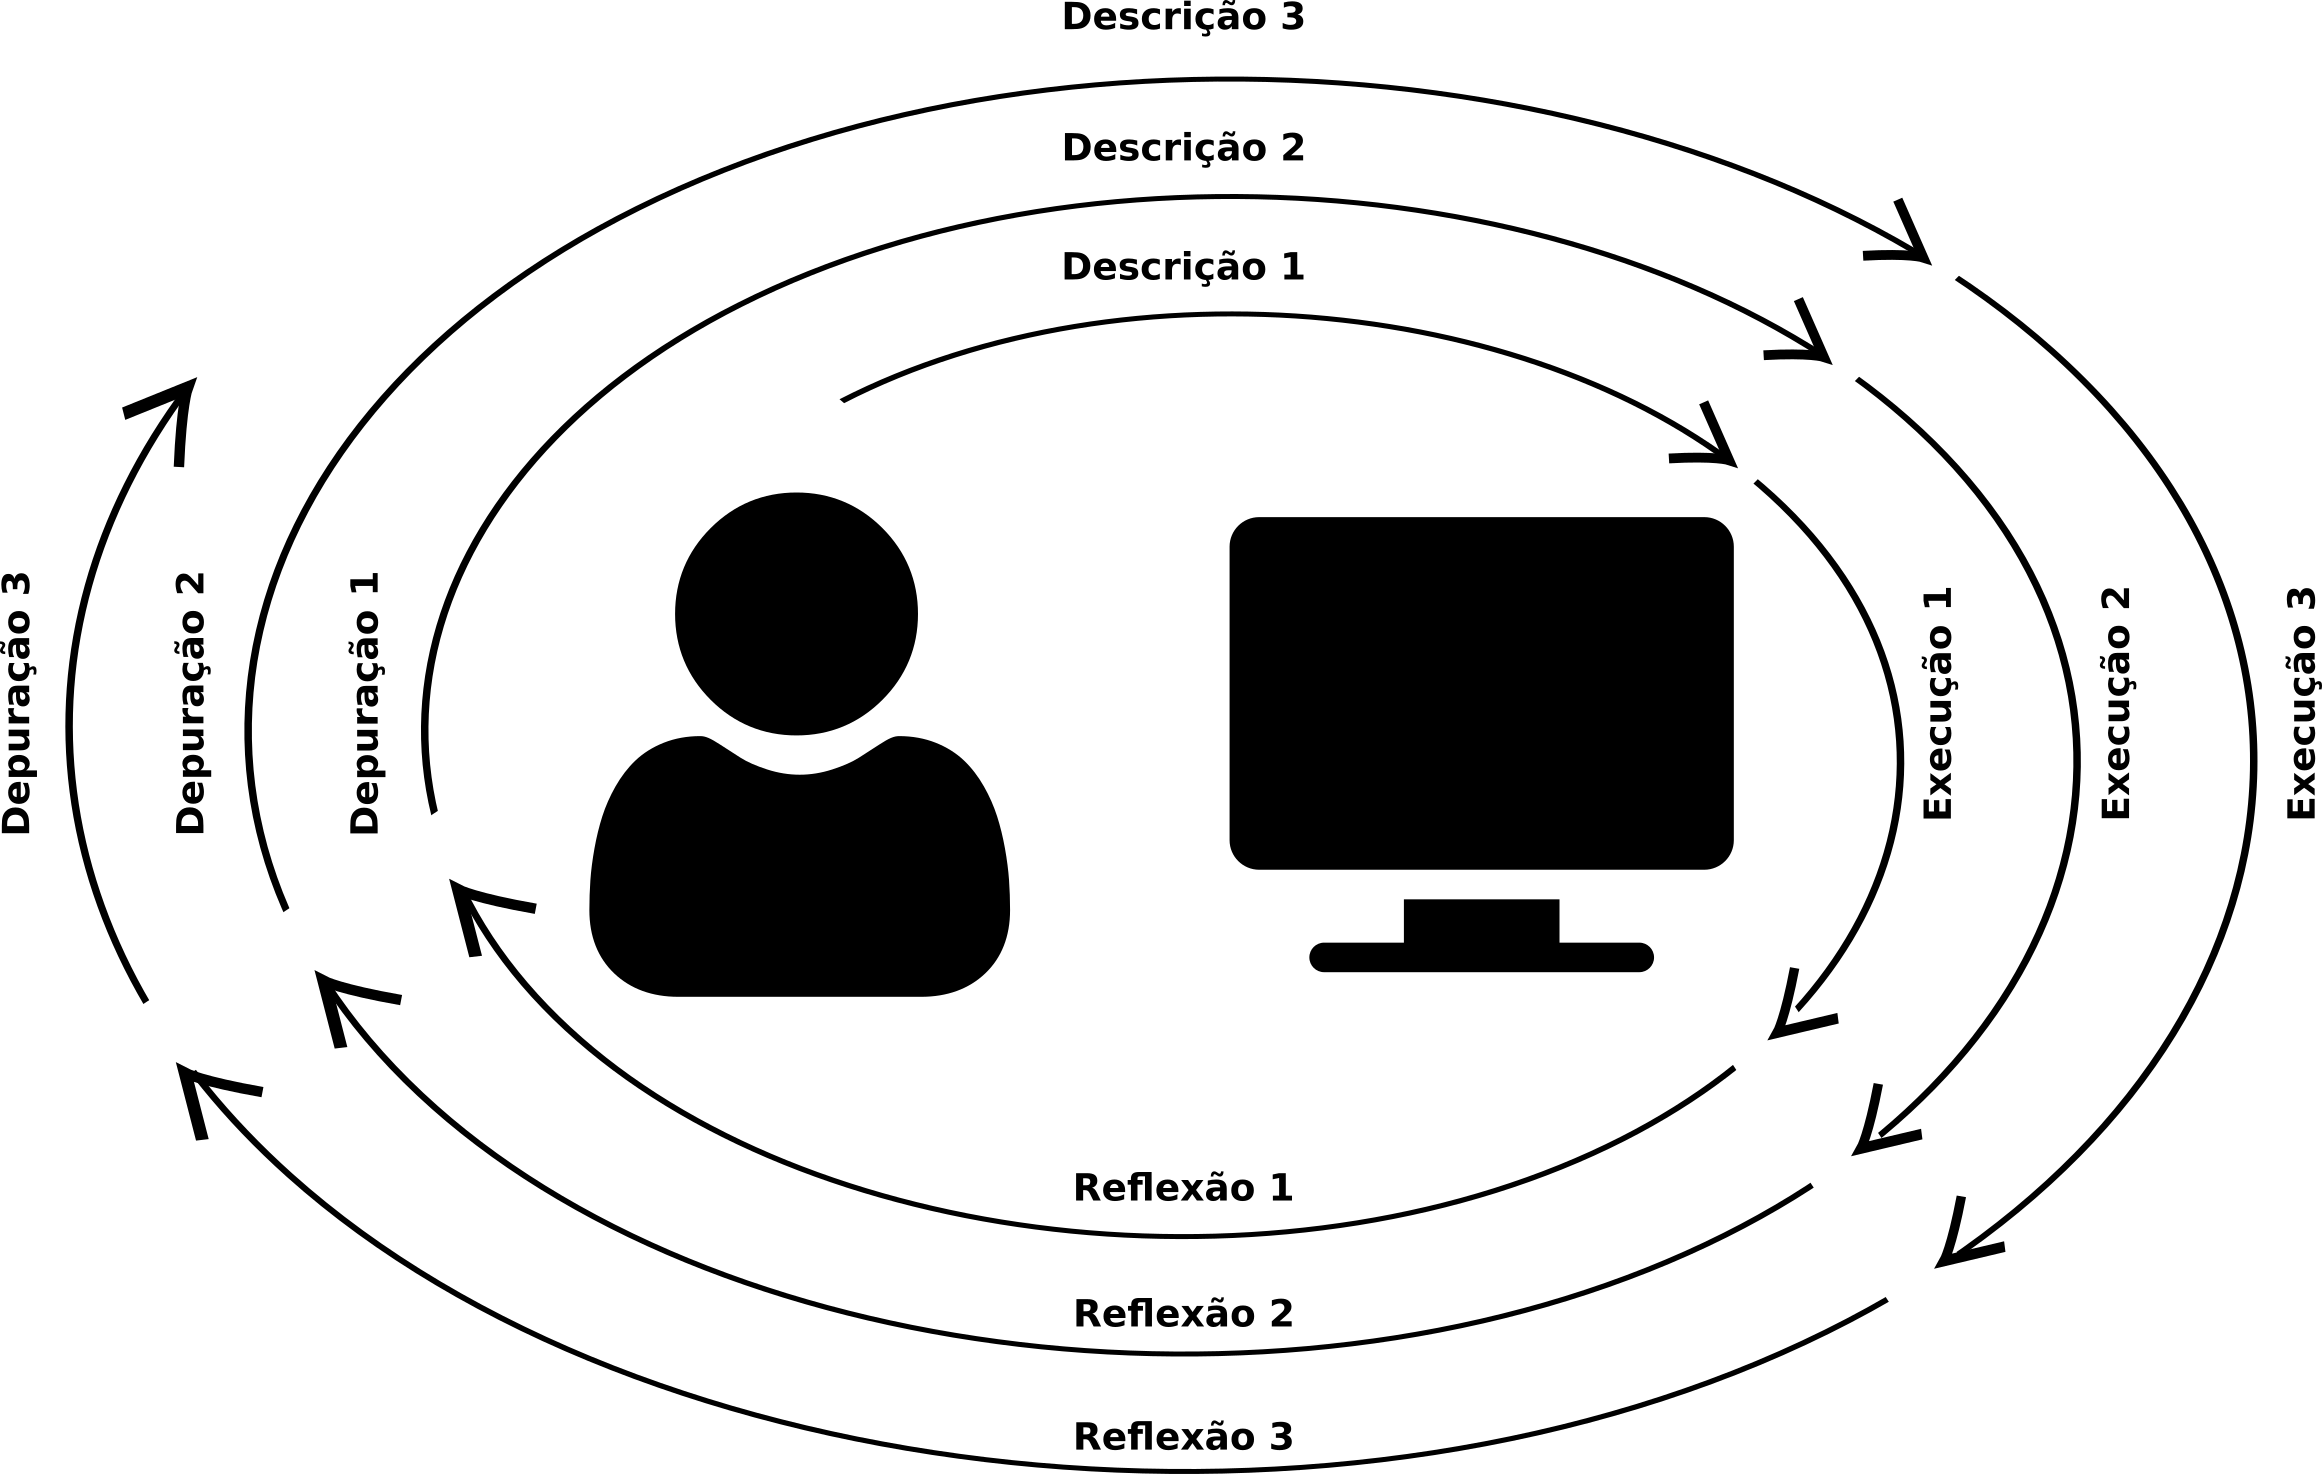
\includegraphics[width=.6\linewidth,fbox]{figs/ciclo_descricao_execucao_reflexao_depuracao.png}
  \caption{Espiral de aprendizagem.}
  \source{Adaptado de \citeonline{valente_aspectos_2018}.}
  \label{fig_espiral}
\end{figure}

A depuração também foi uma das diretrizes de design do ambiente de programação Logo \cite{solomon_history_2020}. Desenvolvido a partir de 1966, ele foi o primeiro ambiente projetado tendo crianças como público-alvo. Era composto por um computador, uma linguagem textual de programação e um robô com rodas capaz de se mover no chão e desenhar sobre papel. Esse ambiente permitia depurar por meio instruções da própria linguagem, como \textit{pause}, impressão de pilha de comandos e impressão de variáveis. 

Além desses recursos técnicos, para \citeonline{solomon_history_2020} a "grande ideia"\ do Logo era permitir à criança depurar seu próprio entendimento do processo computacional e do algoritmo que deveria ser implementado. Um exemplo é o entendimento dos comandos \textit{left} e \textit{right}, que as crianças confundiam com mover para o lado. Para auxiliar a criança depurar esse conceito, um professor poderia sugeri-la "brincar de ser programada", para então compreender que na verdade esses comandos representam movimentos de giro.

A ideia de que a depuração poderia representar uma atividade benéfica para o desenvolvimento cognitivo, somada à existência da linguagem Logo, estimulou pesquisas sobre a depuração por crianças. \citeonline{carver_assessing_1986} avaliaram a depuração de algoritmos por crianças de 7 a 8 anos durante um curso usando Logo. Para isso definiram um modelo de depuração em quatro fases: (i) identificação da diferença entre resultado esperado e resultado obtido; (ii) levantamento de hipóteses para a causa do erro; (iii) localização do \bug\ no código; e (iv) correção do \bug. Com base neste modelo, os pesquisadores concluíram que, após 24 horas de curso, as crianças não desenvolveram estratégias efetivas de depuração, preferindo apagar tudo e reiniciar à procurar \textit{bugs} nos programas. Em estudo posterior, porém, os mesmos autores conseguiram identificar que crianças aprenderam a isolar a procura por bugs e transferiram esta habilidade para atividades não relacionadas à programação \cite{carver_improving_1987}.

Além de possibilitar pesquisas sobre como as crianças programam, o ambiente Logo contribuiu para o surgimento, na década de 1990, de um ramo de estudos de \ac{IHC} focado no design de interação para crianças \cite{hourcade_child-computer_2015}. Inicialmente as crianças programavam em Logo utilizando teclados convencionais, projetados para adultos. Mas como ficou evidente para os pesquisadores, crianças antes dos 10-14 anos de idade não estavam preparadas pra esse tipo de interação \cite{mcnerney_turtles_2004}. O uso dos teclados exigia alfabetização, coordenação motora fina, e propiciava a ocorrência de erros sintáticos. Por isso a criança despendia esforço cognitivo tentando entender o funcionamento da interface, em vez de dedicar-se a desenvolver ideias.

O reconhecimento dessa inadequação na interação das crianças com o ambiente de programação, motivou a criação de uma classe de ferramentas chamada de \ac{BPs}. Os \ac{BPs} descendem do ambiente Logo e buscam facilitar o aprendizado de programação pelo público infantil. Assim como o robô do ambiente Logo, eles geralmente se movem sobre o chão, e tem aparências que remetem ao imaginário infantil, como animais, carros ou robôs \cite{raabe_2017_rope}. Em geral, sua principal funcionalidade é possibilitar à criança inserir comandos, que o brinquedo então executa. Esses brinquedos tem interfaces de programação projetadas para facilitar à criança concentrar-se nos conceitos fundamentais, sem se distrair com erros que não contribuem para o aprendizado de algoritmos.

Considerando que os \ac{BPs} descendem do Logo, espera-se que herdem o princípio de permitir depurar os algoritmos. A preocupação em criar interfaces que facilitem a depuração está presente em ambientes de desenvolvimento profissionais e/ou voltados para o ensino de programação introdutória para adultos. Esses ambientes mostram valores de variáveis na memória, permitem executar passo a passo e definir \textit{break points} \cite{noschang_portugol_nodate}. Se adultos precisam destas ferramentas, será que as crianças poderiam se beneficiar das mesmas funcionalidades caso aplicadas em interfaces de \ac{BPs}?

No contexto dessa pergunta, \citeonline{sipitakiat_robo-blocks_2012} desenvolveram o Robo-Blocks, uma interface tangível de programação em blocos que permite executar passo a passo as instruções de um BP. Eles perceberam a necessidade dessa função ao observar que as crianças tendiam a implementar "grosseiramente"\ suas ideias para ver o robô executá-las, até obter o resultado desejado. Além disso, o robô executava rapidamente e as crianças precisavam escolher olhar para o brinquedo ou para os blocos, dificultando associar um movimento errado com sua causa no código. Com a execução passo a passo as crianças puderam associar blocos com movimentos, o que foi auxiliado por um LED ativado em cada bloco durante sua execução. Outra ferramenta que apresenta certa função de depuração é o Cubetto \cite{anzoategui_cubetto_2017} (\autoref{fig_cubetto}).  Esse brinquedo é programado por um painel no qual são encaixados blocos de madeira. Assim como o Robo-Blocks, o painel destaca cada bloco executado acendendo LEDs.

Uma característica comum nestes trabalhos é a presença de componentes eletrônicos específicos. Tanto os blocos do Robo-Blocks quanto o painel do Cubetto tem um \textit{hardware} com baterias, conectores e placas projetadas para acender luzes conforme o brinquedo executa os comandos. Como alternativa independente de \textit{hardware} \citeonline{fincher_tangible_2019} apresentam as "linguagens externamente compiladas". Elas são interfaces com blocos tangíveis contendo marcas especiais. Essas marcas são lidas por um sensor óptico (câmera ou escâner) e interpretadas por um software externo que identifica as marcas e as "compila"\ de forma compreensível para um agente computacional (geralmente um robô) executar. Os blocos contém pouco ou nenhum componente eletrônico, o que segundo \citeonline{fincher_tangible_2019} dá mais liberdade aos projetistas para escolherem os materiais ou objetos a utilizar. Um exemplo de BP que utiliza interface tangível externamente compilada é o KIBO \cite{sullivan_kibo_2015} (\autoref{fig_kibo}).

\begin{figure}[!htbp]
    \centering
    \begin{subfigure}{.5\textwidth}
        \centering
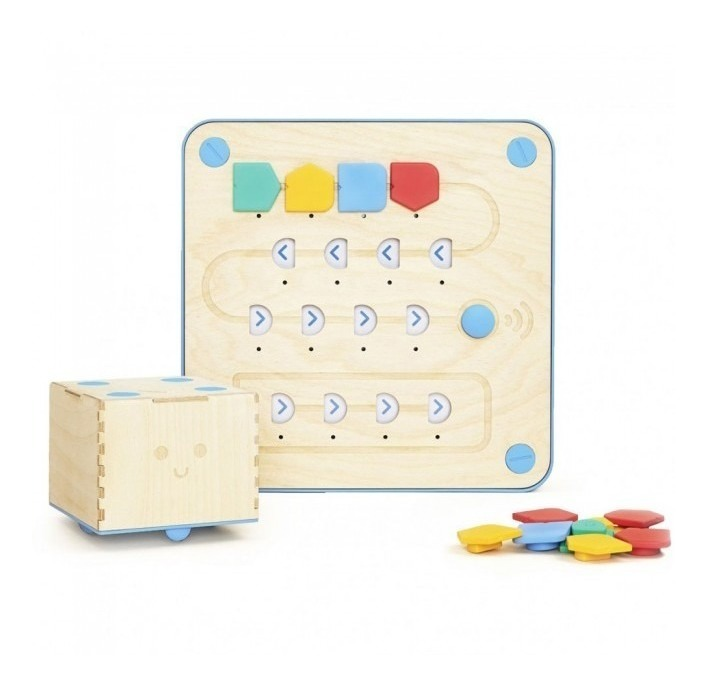
\includegraphics[width=.9\linewidth,fbox]{figs/cubetto.jpg}
        \caption{Cubetto}
        \label{fig_cubetto}
    \end{subfigure}%
    \begin{subfigure}{.5\textwidth}
        \centering
        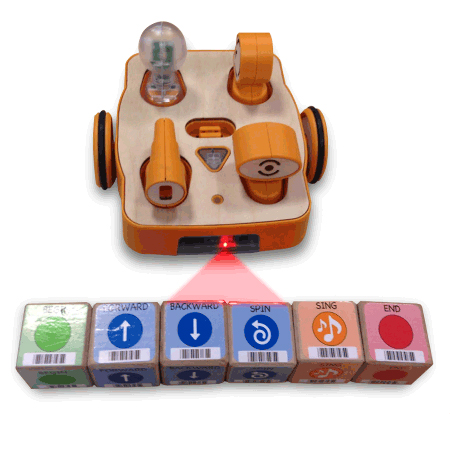
\includegraphics[width=.9\linewidth,fbox]{figs/kibo_2.jpeg}
        \caption{KIBO}
        \label{fig_kibo}
    \end{subfigure}
    \caption{Brinquedos com interfaces tangíveis.}
    \label{fig_toys_tangible}
\end{figure}

%Este trabalho divide as interfaces dos \ac{BPs} dois tipos principais: tangíveis e virtuais. Enquanto as interfaces tangíveis permitem programar por meio de blocos físicos, como o KIBO \cite{sullivan_kibo_2015}, ou botões acoplados ao corpo do brinquedo, como a Bee-Bot\textsuperscript{\textregistered}, as interfaces virtuais permitem ver o algoritmo em uma tela bidimensional. Este segundo grupo inclui dispositivos de toque como \textit{smartphones} e \textit{tablets}, e computadores onde a interação ocorre por teclado e mouse. A \autoref{toy_samples} demonstra quatro exemplos.

Por outro lado, sem componentes eletrônicos como LEDs, os blocos carecem de mecanismos de depuração, ou seja, uma forma de acompanhar o código em execução. A falta de um indicador dificulta para a criança saber qual comando está sendo executado em cada ação do brinquedo, e portanto encontrar causas de erros, bem como fazer o mapeamento entre símbolo (imagem presente no bloco) e ação (realizada pelo brinquedo).

Esse tipo de problema é aderente ao uso de realidade aumentada (RA) projetiva \cite{roberto_dynamic_2013}. Essa técnica permite projetar elementos virtuais sobre objetos reais de modo dinâmico. Enquanto componentes eletrônicos seriam fixos em blocos com baterias ou inseridos em um painel, como o Cubetto, a projeção permite variar as cores e formas projetadas. Deste modo, os blocos tangíveis do algoritmo podem ser construídos com materiais diversos e ainda assim proporcionar \textit{scaffolding} durante a depuração.

O RoPE (Robô Programável Educacional) representa uma oportunidade para testar a viabilidade desta abordagem de criação de interfaces tangíveis externamente compiladas e com uso de RA projetiva. Ele é um BP desenvolvido na Univali pelo Laboratório Lite\footnote{\url{https://lite.acad.univali.br}} com foco em crianças a partir dos 3 anos de idade. A sua interface de programação são botões coloridos (\autoref{fig_rope}), desenhados para serem simples de usar por crianças pequenas \cite{raabe_2017_rope}. Essa interface se mostrou um sucesso, e o brinquedo já foi usado em Centros de Desenvolvimento Infantil por mais de 1000 crianças. Além dos botões, pesquisas desenvolveram protótipos de outros modos de interação, como um aplicativo de celular \cite{viana_cesar_interface_2018} e uma interface de programação em blocos eletrônica \cite{metzger_desenvolvimento_2018}.

%\begin{figure}[!htpb]
  %\centering
  %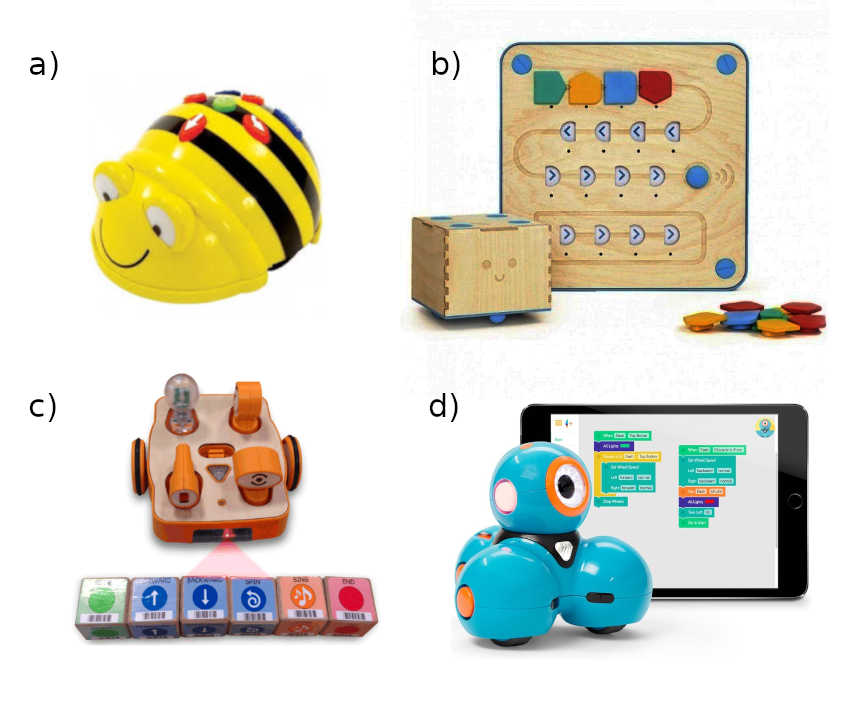
\includegraphics[width=.6\linewidth,fbox]{figs/toys.png}
  %\caption{Exemplos de brinquedos programáveis. a) %Bee-Bot\textsuperscript{\textregistered}; b) Cubetto; c) KIBO; d) Dash}
  %\label{toy_samples}
%\end{figure}

\begin{figure}[!htbp]
    \centering
    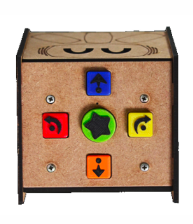
\includegraphics[width=.3\linewidth,fbox]{figs/rope_top.png}
    \caption{Brinquedo RoPE.}
    \label{fig_rope}
\end{figure}

%, e tem duas interfaces: uma interface tangível com 5 botões coloridos, e uma interface virtual via aplicativo \cite{viana_interface_2018}. O brinquedo é distribuído em Centros de Desenvolvimento Infantil (CDI), e tema de pesquisas de graduação \cite{pinheiro_alise_2016, metzger_desenvolvimento_2018} e mestrado \cite{martins_desenvolvimento_2016}. O presente trabalho ocorre no contexto dessas pesquisas, com foco no desenvolvimento e avaliação de interfaces alternativas para crianças de 4 a 6 anos\footnote{A observação de crianças com mais de 6 anos interagindo com o RoPE demonstra que as mesmas tem facilidade. Por isso este trabalho foca na faixa etária mais jovem.}.

Este trabalho ocorre como uma continuidade das duas pesquisas citadas e busca contribuir com a área de Informática na Educação ao (1) projetar uma interface tangível externamente compilada para o brinquedo RoPE e (2) explorar o uso de RA projetiva como um meio de facilitar a depuração. Essa contribuição se fundamenta na literatura em favor das interfaces tangíveis para crianças \cite{sapounidis_evaluating_2015, fincher_tangible_2019, plowman_interactivity_2004} e na observação de que o uso de RA projetiva é um campo inexplorado no contexto de BPs.

%Atualmente os avanços de hardware e técnicas de software tem possibilitado novas alternativas de interação, e isso tem instigado pesquisas que buscam projetar e avaliar essas interfaces \cite{sakamoto_code_2019, burleson_active_2018, sapounidis_evaluating_2015}. Além disso um grande número de novos brinquedos programáveis tem surgido \cite{catlin_edurobots_2018}, levantando o questionamento se ainda seguem os princípios seminais da linguagem LOGO\footnote{Os princípios estão ligados a facilidade de iniciar a programar, mas grande poder naquilo que pode ser criado, denominado "low floor, high ceiling".}.

\section{Problema de Pesquisa} \label{s_cintro_problema_pesquisa}

O problema que este trabalho tenta resolver no campo das interfaces tangíveis de programação é o que \citeonline{norman_design_1988} denomina falta de \textit{visibilidade}. A visibilidade é um princípio de design que permite ao usuário compreender como interagir com determinada interface, e como os resultados das interações devem ser mostrados (\textit{feedback}). A visibilidade (ou a falta dela) também influencia no modelo mental que o usuário cria sobre o funcionamento do objeto com o qual interage.

Em BPs que possuem apenas botões, como o RoPE e a Bee-Bot, ocorre a falta de visibilidade do algoritmo. Não há \textit{visibilidade de estrutura} para a criança perceber o que é um algoritmo, pois a mesma não vê o algoritmo que está construindo ao apertar os botões. Essa falta de visibilidade impede conversar sobre o algoritmo, analisá-lo, encontrar erros e desfazer operações. \citeonline{raabe_brinquedos_2015} relata a falta de compreensão do funcionamento do botão de limpar a memória da Bee-Bot. Uma possível razão para essa falta de compreensão é o fato da memória não estar visível para que se saiba que foi limpa.

No caso das interfaces de blocos tangíveis externamente compiladas (como a utilizada pelo KIBO), o problema é a falta de \textit{visibilidade de execução} do algoritmo. Os blocos carecem de indicadores que mostrem à criança qual bloco está sendo executado em cada momento. Essa falta de visibilidade de execução dificulta compreender a sequência lógica de funcionamento do algoritmo, pois não há mapeamento entre comando/bloco e ação do robô.

\citeonline{norman_design_1988} comenta que a visibilidade influencia o modelo mental que o usuário cria ao interagir com alguma interface. Caso exista falta de visibilidade, e o objeto executar de forma inesperada, o usuário tende a encontrar explicações para justificar tal comportamento. Neste momento, cria um modelo mental errôneo de como o objeto funciona. Um modelo mental errôneo sobre o funcionamento de um BPs pode prejudicar o aprendizado de programação. Isso ocorre em \citeonline{raabe_brinquedos_2015}, onde as crianças não compreenderam a necessidade de usar o botão de limpar a memória (devido à falta de visibilidade) e justificaram o comportamento inesperado do robô afirmando que a abelha tinha vontade própria.

Por fim, essa falta de visibilidade desencadeia a dificuldade em depurar. Os modelos de depuração presentes na literatura \cite{carver_assessing_1986, mccauley_debugging_2008} possuem etapas de localização e reparação de bugs, o que exige acesso à estrutura do algoritmo. Ao não ver essa estrutura ou não acompanhar a sequência de execução dos comandos, acredita-se que a depuração é prejudicada.

A partir destas reflexões elaborou-se a seguinte pergunta de pesquisa:
\textit{Como a visibilidade de algoritmo de um brinquedo programável influencia a prática da depuração de algoritmos por crianças?}

%Por outro lado, as interfaces tangíveis (TUIs) externamente compiladas são compostas de blocos sem componentes eletrônicos. Essa ausência de luzes ou alguma forma automática de indicar que o bloco está sendo executado

%\citeonline{newhouse_programmable_2017} observaram em um estudo que, sem auxílio, crianças não demonstraram ações que pudessem ser associadas a compreensão de "algoritmos".

% giro
%Pesquisas sobre a interação de crianças com brinquedos programáveis mencionam algumas dificuldades. Em pesquisa com a Bee-Bot \cite{raabe_brinquedos_2015} os autores comentam incompreensão do movimento de giro. Girar significa manter-se no mesmo local e deslocar-se sobre o próprio eixo. Porém o movimento é confundido com mudar de posição, ou seja, girar e andar para frente, como o movimento de um carrinho por exemplo.

% lateralidade
%Outra dificuldade é em relação à lateralidade. Devido ao egocentrismo \cite{piaget_representacao_1981}, a criança não consegue imaginar-se em outro ponto de vista. Os comandos que a criança fala são relativos à posição dela. Se o brinquedo está de lado para a criança, e precisa avançar para o próximo quadrante, então a criança diz para ele ir "para o lado", em vez de avançar.

%As interfaces tangíveis e virtuais possuem algumas subcategorias: botões, elementos de auxílio, aplicativos, e blocos tangíveis. Cada uma dessas subcategorias tem vantagens e desvantagens (\autoref{quadro_vantagem_desvantagem}). 

%Os botões são pontos de interação acoplados ao corpo do brinquedo. A vantagem disso é que os símbolos de setas estão na mesma orientação do brinquedo ao programá-lo. A desvantagem é não possuir um visor que demonstre a sequência de comandos programados.

%Os elementos de auxílio são cartas que visam permitir a ver o algoritmo programado. A vantagem é que são tangíveis e baratos. Entretanto não há sincronia com o brinquedo, ou seja, um algoritmo mostrado por cartas pode não corresponder à programação feita no brinquedo.

%Os aplicativos resolvem o problema da sincronia. Por meio de conexão sem fio, permitem programar e ver os comandos programados. A desvantagem é que a experiência de usar telas bidimensionais não é natural, e, além disso, esses dispositivos são de uso pessoal e isso dificulta a colaboração.

%Os blocos tangíveis resolvem o problema da colaboração. Várias crianças podem organizar blocos de madeira ao mesmo tempo. A dificuldade com este tipo de abordagem é a depuração. É difícil projetar blocos que indiquem quando estão em execução. Alternativas para isso são painéis como o do Cubetto, porém o custo destas soluções nem sempre é viável.

\begin{comment}
    \begin{quadro}[!htbp]
 \caption{Vantagens e desvantagens de botões, cartas, tangíveis e aplicativos}
 \label{quadro_vantagem_desvantagem} 
 \begin{center}
 \begin{footnotesize} 
\begin{tabular}{|p{3cm}|p{3cm}|p{4.5cm}|p{4.5cm}|}
\hline
Tipo de interface & Exemplos            & Vantagens & Desvantagens\\ \hline
Botões            & RoPE, Bee-Bot       & - Facilidade de inserir comandos & - Não mostra algoritmo. \newline 
                                                                             - Não permite editar comandos, somente apagar tudo e recomeçar.
\\ \hline
Cartas            & Bee-Bot, \newline
                    Go-Robot Mouse      & - Baixo custo \newline                
                                          - Permite colaboração \newline
                                          - Customizável \newline           & - Falta de sincronia \newline 
\\ \hline
Aplicativos       & Dash, Sphero        & - Sincronia \newline 
                                          - Baixo Custo \newline
                                          - Replicabilidade \newline
                                          - Depuração \newline              & - Tempo de tela \newline
                                                                              - Difícil colaboração

\\ \hline
Blocos tangíveis  & Cubetto, KUMIITA    & - Experiência sensorial
                                          - Colaborativo \newline   
                                          - Algoritmo visível \newline      & - Custo
\\ \hline
                                        
\end{tabular}
 
 \end{footnotesize}
 \end{center} 
 \sourceauthor
\end{quadro}
\end{comment}

%Considerando, então, (i) as dificuldades de compreensão do giro e (ii) as vantagens e desvantagens das interfaces existentes, a questão problema deste trabalho é \textit{como construir uma interface de programação para um brinquedo programável, que tenha as vantagens das interfaces virtuais e tangíveis existentes?}.

\subsection{Solução Proposta}
\label{ss_cintro_solucao}

A proposta é desenvolver uma interface de \ac{RA} projetiva combinada com uma linguagem externamente compilada. Dado que os blocos de linguagens externamente compiladas tem marcas especiais de fácil identificação, chamadas de marcas fiduciais, uma câmera pode captar as posições dos blocos e um algoritmo pode controlar um projetor de modo a destacá-los. Graficamente, a proposta é apresentada na \autoref{idea}.
\begin{figure}[!htpb]
  \centering
  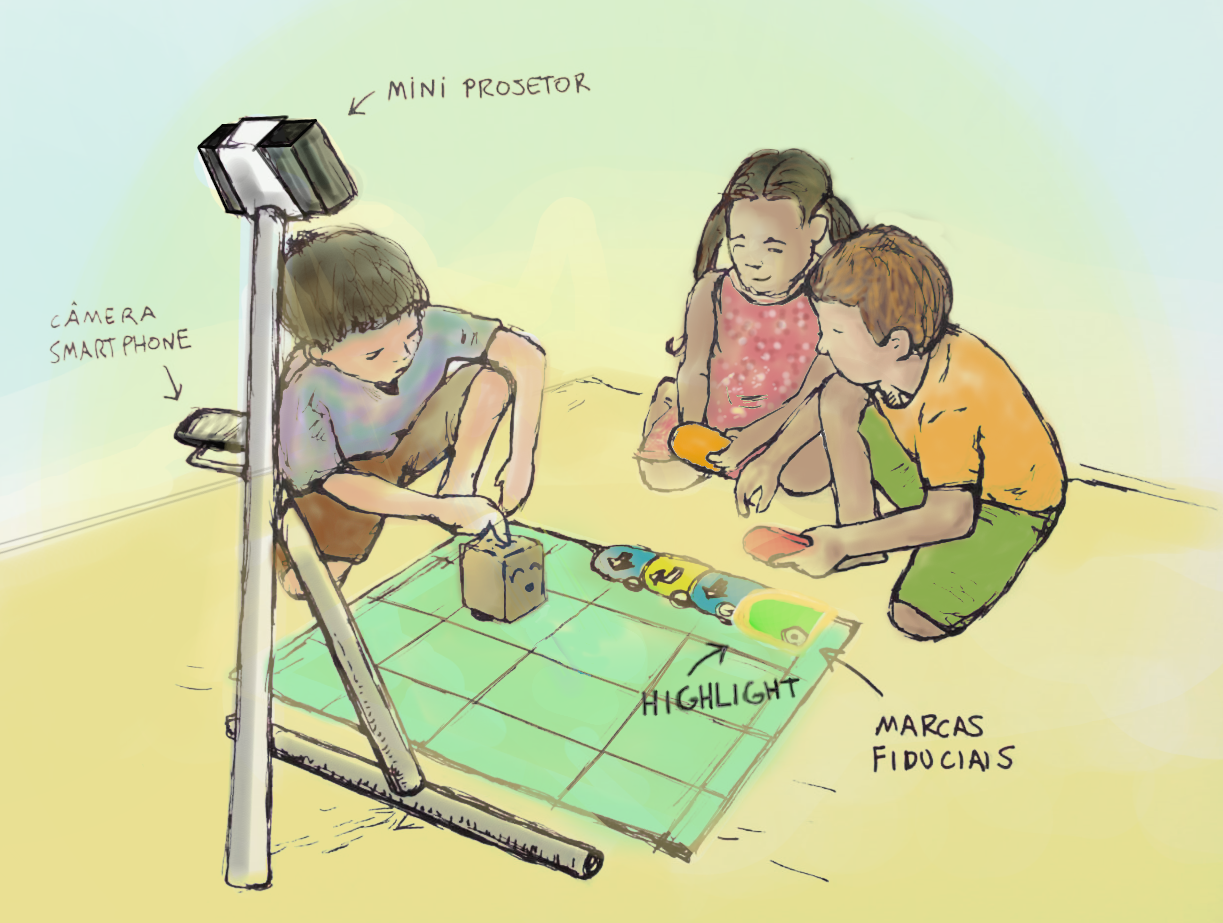
\includegraphics[width=.85\linewidth,fbox]{figs/idea_2.png}
  \caption{Solução proposta: interface tangível com realidade aumentada.}
  \sourceauthor
  \label{idea}
\end{figure}

A intenção é que a criança programe utilizando blocos de papelão com símbolos de setas correspondentes às ações do RoPE. O dispositivo externo com câmera é um \textit{smartphone}, dado que é mais acessível e fácil de manusear do que um laptop ou desktop. O projetor utilizado é portátil e de baixa potência de iluminação (1200 lumens), o que diminui o seu custo.

Outra funcionalidade a ser implementada é a execução passo a passo. Para isso, a criança utilizará uma seta especial que será colocada ao lado da sequência de comandos, apontando para um bloco. Para que o próximo comando seja executado, a seta deve ser movida para ele. Deste modo, a criança deve mover a seta apontando para cada bloco até o fim da sequência, reforçando o mapeamento entre símbolo e ação e facilitando a depuração.

Com a construção dessa ferramenta, pretende-se avaliar qualitativamente as interações de crianças de 4 a 6 anos com a mesma. 

\subsection{Delimitação de Escopo}
\label{ss_cintro_escopo}

Este trabalho se insere no contexto de ferramentas que buscam permitir o aprendizado de algoritmos por crianças. Na definição de \citeonline{brackmann_desenvolvimento_2017}, algoritmos é um dos pilares do \acl{PC} \cite{brackmann_desenvolvimento_2017}, que tem outros três pilares: decomposição, abstração e reconhecimento de padrões. Este trabalho cita as definições destes pilares, porém a solução proposta tem foco apenas no pilar algoritmos e mais especificamente na atividade de depurá-los.

Não se pretende realizar testes com objetivos de comprovação estatística, no sentido de efeitos para o aprendizado. O foco é avaliar aspectos de usabilidade, descrevendo a ocorrência ou ausência das dificuldades mais perceptíveis durante a programação. A avaliação ocorrerá com um número reduzido de crianças, com objetivo de avaliar mais profundamente aspectos qualitativos.

Também não é objetivo programar um algoritmo de visão computacional para reconhecer os blocos tangíveis e o RoPE. A intenção é utilizar marcadores a biblioteca de identificação de marcas fiduciais denominada TopCodes\footnote{\url{http://users.eecs.northwestern.edu/~mhorn/topcodes/}} para agilizar a implementação e validar a proposta. Caso a usabilidade da proposta se confirme, então a eliminação de marcas fiduciais poderá ocorrer em trabalhos futuros.

% ----------------------------------------------------------------------- %
\subsection{Justificativa}
\label{ss_cintro_justificativa}

Em um mapeamento industrial descrito no \autoref{c_estado_arte}, foi identificado que, de 56 brinquedos, apenas 2 utilizam RA. Ainda assim o seu uso ocorre por meio de dispositivos móveis com interface gráfica, que são menos adequados para crianças em comparação com as interfaces tangíveis \cite{sapounidis_tangible_2019, zuckerman_tui_2013}.

%No Brasil há poucas pesquisas relacionadas à computação com foco na Educação Infantil \citeonline{gomes_jogos_2016}. Apesar deste tema ter ganhado destaque em países da Europa, na Austrália e nos Estados Unidos, no Brasil ele ainda é um esforço de alguns pesquisadores e grupos. 

O brinquedo RoPE é um dos poucos exemplos acadêmicos de ferramentas educacionais brasileiras voltadas ao ensino de programação para crianças pequenas. Desde sua concepção há uma preocupação com aspectos de design para que crianças possam aprender de forma lúdica evitando erros não construtivos \cite{raabe_brinquedos_2015}. O tipo de interação proposto neste trabalho ainda não foi experimentado, tanto com o RoPE quanto em outros brinquedos, e portanto a sua exploração contribuir com novas informações para a área.

O fato da solução proposta não utilizar um hardware específico, ou seja, usar apenas produtos disponíveis comercialmente por mais de um fabricante (mini-projetores e \textit{smartphones}), facilita aplicar a solução a outros brinquedos. O RoPE compartilha características com uma classe de brinquedos, como a Bee-Bot, Go Robot Mouse e Thymio, e que poderiam testar a proposta apresentada.

O \autoref{c_desenvolvimento} apresenta a viabilidade da solução. A qualidade de imagem gerada por um projetor de baixo custo é aceitável em ambientes iluminados artificialmente, como salas de aula, museus e bibliotecas. Ambientes externos exigem maior potência de iluminação e não foram avaliados.

A proposta de usar realidade aumentada projetiva abre caminho para desenvolver tapetes dinâmicos. Atualmente o brinquedo RoPE se move sobre tapetes estáticos, que precisam ser trocados de acordo com a atividade. O fato de projetar o ambiente do brinquedo, associado à informação de sua localização, permite criar eventos disparados quando o brinquedo chega em determinada posição do tapete. É possível até mesmo construir jogos com diversas fases, que avançam conforme o brinquedo se move. Portanto, ao permitir que um sistema computacional perceba a posição do brinquedo e projete o ambiente, surgem novas possibilidades de interação.

Entretanto, antes que essas novas possibilidades sejam alcançadas é preciso avaliar a usabilidade da ferramenta. Há riscos, como a obstrução das marcas fiduciais, e o excesso de elementos que poderiam distrair a criança. O teste com crianças permitirá aprender sobre esses riscos e indicar a viabilidade dessa abordagem em ambientes reais.

Concluindo, a proposta está ligada à uma área de interesse da comunidade científica \footnote{Possui jornais dedicados ao tema, como International Journal of Child-Computer Interaction e ACM Transactions on Computer-Human Interaction.}, e haver uma lacuna de compreensão sobre utilização de realidade aumentada projetiva com brinquedos programáveis.

\section{Objetivos}
\label{s_cintro_objetivos}

\subsection{Objetivo Geral}
\label{ss_cintro_objetivo_geral}

Avaliar qualitativamente o uso de uma interface de realidade aumentada projetiva na depuração de algoritmos por crianças de um Centro de Desenvolvimento Infantil.

\subsection{Objetivos Específicos}
\label{ss_cintro_objetivos_espec}

O trabalho pretende contribuir com o campos de design de interação e educação em computação ao:

\begin{enumerate}
    
    \item Apresentar aplicações de RA projetiva;

    \item\label{obj_mapear} Mapear os principais tipos de interfaces de brinquedos programáveis existentes;
    
    \item\label{obj_interface} Construir a interface de realidade aumentada projetiva para o brinquedo RoPE;
    
    \item\label{obj_avaliar} Experimentar a interface em atividades com crianças e coletar eventos de interação.
    
\end{enumerate}
\section{Metodologia}
\label{s_cintro_metodologia}

Esta seção descreve a metodologia e os procedimentos metodológicos utilizados nesta pesquisa.

\subsection{Métodos da Pesquisa}
\label{ss_cintro_metod_pesquisa}

\citeonline{gil_metodos_2008} define método científico como um conjunto de procedimentos técnicos adotados para produzir conhecimento. \citeonline{wazlawick_metodologia_2009} comenta que o método científico é uma sequência de passos demonstrando como atingir os objetivos de pesquisa. Os métodos científicos tem duas características: os procedimentos técnicos e as bases lógicas de raciocínio que guiam a investigação.

Quanto aos procedimentos técnicos, esta pesquisa tem natureza aplicada, pois prevê a utilização prática de uma ferramenta e tecnologias específicas para solucionar um problema de interação com brinquedos programáveis.

A abordagem sobre esse problema foi qualitativa, ao observar aspectos subjetivos como falas, gestos e expressões durante o uso da solução proposta. Por fim, esta pesquisa tem objetivos exploratórios, ao buscar extrair informações dos dados coletados em um .

\subsection{Procedimentos Metodológicos}
\label{ss_cintro_proced_metodologicos}

A construção da solução proposta e atendimento dos objetivos de pesquisa possui quatro fases: estudo, modelagem, implementação e avaliação.

A etapa de estudo\footnote{Etapa realizada para atender o objetivo específico \autoref{obj_mapear}. } correspondeu a uma revisão sistemática, um mapeamento industrial e um levantamento de trabalhos similares. A revisão sistemática focou em compreender como são feitas pesquisas científicas avaliando interfaces de programação de brinquedos programáveis. O mapeamento, por sua vez, buscou descrever quais tipos de interfaces são utilizadas em projetos comerciais de brinquedos programáveis. Por último, os trabalhos similares descrevem o uso de projeção ou formas de facilitar a programação por crianças.

A etapa de modelagem é descrita no \autoref{c_desenvolvimento}, onde é apresentado o planejamento dos elementos de software a serem implementados. Para isso foi utilizado técnicas padrão, como diagrama de classes, levantamento de requisitos e desenho de telas.

A etapa de implementação\footnote{Etapa realizada para atender o \autoref{obj_api} e o \autoref{obj_interface} dos objetivos específicos} correspondeu a programar quatro elementos: (i) uma \ac{API} para captação e armazenamento das interações ocorridas com um brinquedo programável; (ii) adaptar o \textit{firmware} do brinquedo RoPE para comunicação sem fio; e (iii) programar um aplicativo de \textit{smartphone} para captar os blocos e comunicar com o projetor.

A avaliação\footnote{ Para atendimento do objetivo específico \autoref{obj_avaliar}.} corresponde a observar crianças programando o brinquedo, e coletar dados seguindo um protocolo definido no \autoref{c_avaliacao}. A ideia nesta etapa é executar estudos de caso, onde se coletará as interações quantitativa meio da \ac{API} e serão registradas informações qualitativas em diário de bordo. A ideia é organizar um processo em que cada caso subsidie melhorias na interface a serem testadas no próximo caso.

%Você deve identificar os procedimentos técnicos que você utilizou, como, por exemplo:

\begin{comment}
    \item Pesquisa bibliográfica;
    \item Pesquisa documental;
    \item Pesquisa experimental;
    \item Levantamento;
    \item Estudo de caso;
    \item Pesquisa ex post facto;
    \item Pesquisa-ação; 
    \item Pesquisa participante; ou
    \item Outros.
\end{comment}

%Você deve definir as etapas utilizadas na execução do seu trabalho, por meio de um plano de trabalho descrito textualmente, explicando as atividades realizadas, os resultados obtidos, os artefatos desenvolvidos, etc. Você deve explorar os procedimentos técnicos comentados na seção anterior. Você deve fazer uma ligação entre as etapas executadas na sua pesquisa e os objetivos específicos da dissertação. Todos os objetivos específicos devem ser atendidos com a execução dos itens do plano de trabalho.

% ----------------------------------------------------------------------- %
\section{Estrutura da Dissertação}
\label{s_cintro_estrutura}

%Nesta seção, deve-se descrever a estrutura do texto, de forma textual, identificando o conteúdo e as contribuições de cada capítulo da dissertação. Abaixo, segue um exemplo de redação a ser utilizada.

O trabalho está organizado em 6 capítulos correlacionados. O \autoref{c_introducao}, Introdução, contextualizou e apresentou o tema, o problema e uma proposta de como solucioná-lo. Foram estabelecidos os objetivos a serem alcançados com a solução as limitações de escopo a serem observadas.

O \autoref{c_fundamentacao_teorica} apresenta a fundamentação teórica iniciando com a descrição do sujeito mais importante desta pesquisa (a criança) e observa aspectos relacionados ao desenvolvimento infantil. Além disso é apresentada a definição de \ac{PC} em quatro pilares, e conceitos presentes nas interfaces de brinquedos programáveis.

O \autoref{c_estado_arte} apresenta o estado da arte em três aspectos: das pesquisas realizadas com brinquedos programáveis; interfaces de brinquedos mais utilizados no mercado; e trabalhos com semelhanças tecnológicas e conceituais.

O \autoref{c_desenvolvimento} apresenta a modelagem dos elementos de software que integram a contribuição: \textit{firmware}, aplicativo e API. O capítulo apresenta tecnologias utilizadas para construir esses componentes e possibilitar a comunicação entre os mesmos.

O \autoref{c_avaliacao} descreve o contexto de execução da pesquisa. O capítulo também apresenta protocolo de teste a ser aplicado, a organização dos dados gerados e as estatísticas a serem aplicadas sobre os dados para responder as hipóteses de pesquisa.

Por fim, o \autoref{c_conclusao} revisa o atendimento aos objetivos da pesquisa, reflete sobre as contribuições geradas até o momento e planeja as próximas etapas do trabalho.

%No Capítulo N, são tecidas as conclusões do trabalho, relacionando os objetivos identificados inicialmente com os resultados alcançados. São ainda propostas possibilidades de continuação da pesquisa desenvolvida a partir das experiências adquiridas com a execução do trabalho.
